\renewcommand{\theequation}{\theenumi}
\renewcommand{\thefigure}{\theenumi}
\renewcommand{\thetable}{\theenumi}
\begin{enumerate}[label=\thesection.\arabic*.,ref=\thesection.\theenumi]
\numberwithin{equation}{enumi}
\numberwithin{figure}{enumi}
\numberwithin{table}{enumi}

\item Let $X_{1}$ and  $X_{2}$ be i.i.d random variables with poisson. Then ($X_{1}+2X_{2}$) is not sufficient because
\begin{enumerate}
    \item{$\pr{X_{1}=1,X_{2}=1 |T=3}$ depends on $\lambda$}\\
    \item{$X_{1}+2X_{2}$ is poisson}\\
     \item{$X_{1}+2X_{2}$ is not poisson}\\
      \item{$\pr{X_{1}=1,X_{2}=1 | T=3}$ is Poisson with parameter one}\\
\end{enumerate}
Where T=($X_{1}+2X_{2}$)
\solution
%\begin{definition}
    Statistic : A statistic is a function T = r($X_{1},X_{2},\dots,X_{n}$) of the random sample $X_{1},X_{2},\dots,X_{n}$.
  \end{definition}
  \begin{definition}
   Sufficient Statistics : A statistic t = T(X) is sufficient for $\theta$ if the conditional probability distribution of data X, given the statistic t = T(X), doesn't depend on the parameter $\theta$.
   \begin{align}
       \pr{\theta \vert T(X)}=\pr{\theta \vert X}
   \end{align}
  \end{definition}
  \begin{theorem}[Factorization theorem]\label{poisson/4/factor}
   : Let $X_{1},X_{2} · · · , X_{n}$ form a random sample from either a continuous
distribution or a discrete distribution for which the pdf or the point mass function is $f(x\vert\theta)$,
where the value of $\theta$ is unknown and belongs to a given parameter space $\Theta$. A statistic
T($X_{1},X_{2} · · · , X_{n}$) is a sufficient statistic for $\theta$ if and only if the joint pdf or the joint point mass
function $f_{n}$(x$\vert\theta$) $X_{1},X_{2} · · · , X_{n}$ can be factorized as follows for all values of $x = (X_{1},X_{2} · · · , X_{n}) \to$
$R^{n}$ and all values of $\theta \in \Theta$:
$f_{n}(x\vert \theta) = u(x)v\brak{T(x), \theta}.$\\
Here the function u may depend on x but does not
depend on $\theta$, and the function v depends on $\theta$ but will depend on the observed value x only through the value of the statistic T(x).
  \end{theorem}
  \begin{lemma} \label{poisson/4/a}
Suppose that $X_{1}$ and $X_{2}$ are i.i.d poisson random variables with parameter $\lambda$, $T=X_{1}+2X_{2}$ does not follow poisson distribution.
\end{lemma}
\begin{proof}
Let $\Phi_{X_{1}}(\omega)$, $\Phi_{2X_{2}}(\omega)$ and  $\Phi_{T}(\omega)$be the characteristic functions of probability density function of random variables $X_{1}$, $2X_{2}$ and T respectively.\\
\begin{align}
    \Phi_{X_{1}}(\omega)=E(e^{i\omega X_{1}})&=\sum_{x=0}^{\infty}\pr{X_{1}=x}e^{i\omega x}\\
                    &=\sum_{x=0}^{\infty}\frac{e^{i\omega x-\lambda}\lambda^{x}}{x!}\\
                    &=e^{-\lambda}\sum_{x=0}^{\infty}\frac{(e^{i\omega}\lambda)^{x}}{x!}\\
                    &=e^{\lambda\brak{e^{i\omega}-1}}
\end{align}
Similarly,
% \begin{multline}
%     \Phi_{2X_{2}}(\omega)=E\brak{e^{i\omega 2X_{2}}}&=\sum_{x=0}^{\infty}\pr{X_{2}=\frac{x}{2}}e^{i\omega x}\\
%                     =\sum_{x=0,2,4....}^{\infty}\frac{\brak{e^{i\omega x-\lambda}}\lambda^{\frac{x}{2}}}{(\frac{x}{2})!}\\
%                     =e^{-\lambda}\sum_{\frac{x}{2}=0,1,2..}^{\infty}\frac{\brak{e^{2i\omega}\lambda}^{\frac{x}{2}}}{(\frac{x}{2})!}\\
%                     =e^{\lambda\brak{e^{2i\omega}-1}}\\
%                     \end{multline}
                    \begin{align}
\Phi_{T}\brak{\omega}&=\Phi_{X_{1}}\brak{\omega}\times\Phi_{2X_{2}}\brak{\omega}\\
 &=e^{\lambda\brak{e^{i\omega}+e^{2i\omega}-2}}\\ 
 &\neq e^{\mu\brak{e^{i\omega}-1}}
 \end{align}
 Hence the characteristic function of T ($\Phi_{T}(\omega)$) is not in the form of the characteristic function of a poisson random variable (for any value of the parameter $\mu$).\\
 \end{proof}
 \begin{lemma}
 Suppose that $X_{1}$ and $X_{2}$ are i.i.d random variables with poisson distribution then T=$X_{1}+2X_{2}$ is not a sufficient statistic.
 \end{lemma}
 \begin{proof}
 Joint p.m.f of $X_{1}$ and $X_{2}$ is,
 \begin{align}
     f_{X_{1}X_{2}}(x_{1},x_{2})&=\frac{e^{-2\lambda}\lambda^{\brak{x_{1}+x_{2}}}}{x_{1}!x_{2}!}\label{poisson/4/a}\\
     &=\frac{1}{x_{1}!x_{2}!}\times\lambda^{T\brak{X_{1},X_{2}}}e^{-2\lambda}\lambda^{-x_{2}}
 \end{align}
 As we can see \eqref{poisson/4/a} cannot be expressed in the form of $u(x)v\brak{T(x), \theta}$\\
 Hence using factorization theorem \ref{poisson/4/factor}, T is not a sufficient statistic. 
 \end{proof}
  \begin{enumerate}
 \item We know T=3 when $(X_{1},X_{2})$ have values (1,1) and (3,0)
  \begin{multline}
\pr{X_{1}=1,X_{2}=1 |T=3}\\&=\frac{\pr{X_{1}=1,X_{2}=1 \cap T=3}}{\pr{T=3}}\\
=\frac{\pr{X_{1}=1,X_{2}=1}}{\pr{X_{1}=1,X_{2}=1}+\pr{X_{1}=3,X_{2}=0}}\\
=\frac{e^{-2\lambda}\lambda^{2}}{e^{-2\lambda}\lambda^{2}+\frac{e^{-3\lambda}\lambda^{3}}{6}}\\
=\frac{6}{6+\lambda}\neq \frac{e^{-1}1^{\lambda}}{\lambda!}
\end{multline}
Hence $\pr{X_{1}=1,X_{2}=1 |T=3}$ depends on $\lambda$ but is not poisson with parameter 1.
$\implies$option 4 is incorrect and option 1 is correct.\\
\item Using lemma $\ref{poisson/4/a}$, $T=X_{1}+2X_{2}$ is not poisson.\\
$\implies$ option 2 is incorrect, option 3 is correct\\

\item Let $X$ be a Poisson random variable with p.m.f
\begin{align}
\label{poisson/1/eq:1}
P(X=k) = 
    \begin{cases} 
      \frac{e^{-\lambda}\lambda^{k}}{k!},& k=0,1,2,...;  \lambda > 0\\
      0 & \text{otherwise}
   \end{cases}
\end{align}
If $Y = X^2 + 3$, then what is $P(Y=y)$ equal to?
\begin{enumerate}[label={(\Alph*)}]
    \item $\frac{e^{-\lambda}\lambda^{\sqrt{y-3}}}{\sqrt{\brak{y-3}}!}$, for $y =$ \cbrak{3,4,7,12,...}
    \item $\frac{e^{-\lambda}\lambda^{-\sqrt{y-3}}}{\sqrt{\brak{3-y}}!}$, for $y =$ \cbrak{3,4,7,12,...}
    \item $\frac{e^{-\lambda}\lambda^{\sqrt{3-y}}}{\sqrt{\brak{3-y}}!}$, for $y =$ \cbrak{4,7,12,...}
    \item $\frac{e^{-\lambda}\lambda^{-\sqrt{3-y}}}{\sqrt{\brak{3-y}}!}$, for $y =$ \cbrak{4,7,12,...}
\end{enumerate}
%
\solution
%
\begin{align}
    Y = X^2 + 3\\
\implies     X = \sqrt{Y - 3}
\end{align}
Substituting $k = \sqrt{y-3}$ in \eqref{poisson/1/eq:1},
\begin{align}
p_Y(y) = 
    \begin{cases} 
      \frac{e^{-\lambda}\lambda^{\sqrt{y-3}}}{\sqrt{\brak{y-3}}!}, & y=3,4,7,12,...\\
      0&\text{otherwise}
   \end{cases}
\end{align}
Hence, the correct option is \brak{A}.
\begin{figure}[hb]
    \centering
    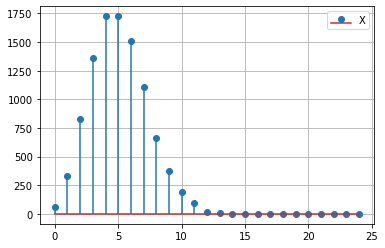
\includegraphics[width=\columnwidth]{poisson/solutions/1/Figures/FigureX.png}
    \caption{Poisson stem plot for X \brak{\lambda = 5}}
    \label{poisson/1/fig:plot1}
\end{figure}
\begin{figure}[hb]
    \centering
    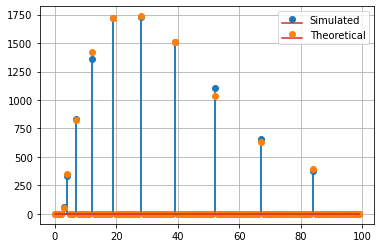
\includegraphics[width=\columnwidth]{poisson/solutions/1/Figures/FigureComp.png}
    \caption{Stem plot for Y (Simulated and Theoretical) \brak{\lambda = 5}}
    \label{poisson/1/fig:plot3}
\end{figure}


\item For $n \geq 1$, let $X_n$ be a Poisson random  variable with mean $n^2$.
 Which of the following are equal to
 $\displaystyle{\frac{1}{\sqrt{2\pi}} \int \limits_2^{\infty} e^{-x^2/2}\,dx}$
\begin{enumerate}
    \item $\lim \limits_{n \to \infty} $ \pr{X_n > (n+1)^2}
    \item $\lim \limits_{n \to \infty} $ \pr{X_n \leqslant (n+1)^2}
    \item $\lim \limits_{n \to \infty} $ \pr{X_n<(n-1)^2}
    \item $\lim \limits_{n \to \infty} $ \pr{X_n<(n-2)^2}
\end{enumerate}
%
\solution
\begin{lemma}
    Let $Y_i$ be a Poisson random variable with mean $1$ for $i$ $\in$ $\brak{1,n^2}$
Then, 
\begin{align}
    \sum \limits_{i}^{n^2} Y_i = X_n   
\end{align}

\end{lemma}
\begin{lemma}
    \begin{align}
         \lim  \limits_{n\to \infty} \frac{X_n-n^2}{n} = \mathcal{N}\brak{0,1}
         \label{poisson/2/central}
    \end{align}
    \label{poisson/2/central/lemma}
\end{lemma}
\begin{proof}
Using the  central limit theorem,
    \begin{align}
        \lim  \limits_{n \to \infty} \frac{Y_1+Y_2+..+Y_{n^2} - n^2}{n} = \mathcal{N}(0,1)
    \end{align}
yielding \eqref{poisson/2/central}.
\end{proof}
\begin{lemma}
    \begin{align}
    Q\brak{2} = \displaystyle{\frac{1}{\sqrt{2\pi}} \int \limits_2^{\infty} e^{-x^2/2}\,dx}
\end{align}
\label{poisson/2/qfunc/lemma}
\end{lemma}
\begin{lemma}
        \begin{align}
            \pr{X_n>k} 
            \\ =& Q\brak{\frac{k-n^2}{n}}
            \label{poisson/2/eq-cdf}
        \end{align}        
        \label{poisson/2/eq-cdf/lemma}
\end{lemma}
\begin{proof}
    For $X \sim \gauss{0}{1}$, using Lemma     \ref{poisson/2/central/lemma},
    \begin{align}
        \pr{X_n>k} 
            =& \pr{X>\frac{k-n^2}{n}}
    \end{align}
    yielding             \eqref{poisson/2/eq-cdf}.
\end{proof}
\begin{lemma}
\begin{align}
    Q\brak{X}=1-Q\brak{-x}
    \label{poisson/2/eq-Qx}
\end{align}
\label{poisson/2/eq-Qx/lemma}
\end{lemma}

% Here, $\mathcal{N}\brak{0,1}$ is normal distribution with unit mean and variance
% Now 
% \begin{align*}
%     \because \,{\frac{1}{\sqrt{2\pi}} \int \limits_{-x}^{\infty} e^{-x^2/2}\,dx}\,=\,{\frac{1}{\sqrt{2\pi}} \int \limits_{-\infty}^x e^{-x^2/2}\,dx}
%     \\ \text{and} \quad \frac{1}{\sqrt{2\pi}} \int \limits_{-\infty}^{\infty} e^{-x^2/2}\,dx\,=1
% \end{align*}
% Also
% \begin{align}
%     \frac{1}{\sqrt{2\pi}} \int \limits_2^{\infty} e^{-x^2/2}\,dx=& Q\brak{2}
% \end{align}
\begin{enumerate}
%\setlength\itemsep{1em}
\item Using Lemma         \ref{poisson/2/eq-cdf/lemma},
\begin{align}
    \lim \limits_{n \to \infty} \pr{X_n > (n+1)^2} =& \lim \limits_{n \to \infty}Q \brak{\frac{(n+1)^2-n^2}{n}}
    \\=&Q\brak{2}
\end{align}
$\mathbf{\therefore}$ \textbf{Option 1 is correct}
\item Using Lemma         \ref{poisson/2/eq-cdf/lemma},
\begin{align}
\begin{split}
    \lim \limits_{n \to \infty} & \pr{X_n \leqslant (n+1)^2}\\ =&1-\lim \limits_{n \to \infty}  \pr{X_n > (n+1)^2}
\end{split}
    \\=&1- \lim \limits_{n \to \infty}Q \brak{\frac{(n+1)^2-n^2}{n}}
    \\=&1- Q \brak{2}
    \\ \ne &  Q\brak{2}
\end{align}
$\mathbf{\therefore}$, from Lemma \ref{poisson/2/qfunc/lemma} \textbf{Option 2 is incorrect}
\item   Using Lemma         \ref{poisson/2/eq-cdf/lemma} and Lemma \ref{poisson/2/eq-Qx/lemma}
\begin{align}
\begin{split}
    \lim \limits_{n \to \infty} & \pr{X_n < (n-1)^2}\\ =&1-\lim \limits_{n \to \infty}  \pr{X_n \geq (n-1)^2}
\end{split}
    \\=&1-\lim \limits_{n \to \infty}Q \brak{\frac{(n-1)^2-n^2}{n}}
    \\=& 1-Q \brak{-2}
    \\=& Q\brak{2}
\end{align}
$\mathbf{\therefore}$ \textbf{Option 3 is also correct}
\item Using Lemma         \ref{poisson/2/eq-cdf/lemma} and Lemma \ref{poisson/2/eq-Qx/lemma},
\begin{align}
   \begin{split}
    \lim \limits_{n \to \infty} & \pr{X_n < (n-2)^2}\\ =&1-\lim \limits_{n \to \infty}  \pr{X_n \geq (n-2)^2}
\end{split}
    \\=&1-\lim \limits_{n \to \infty}Q \brak{\frac{(n-2)^2-n^2}{n}}
    \\=&1- Q \brak{-4}
    \\=& Q\brak{4} < Q \brak{2}
\end{align}
$\mathbf{\therefore}$ \textbf{Option 4 is incorrect}
\end{enumerate}

%
%
\solution
\begin{definition}\label{poisson/3/poisson_process}
    (Poisson Process)\\
    A counting process (number of arrivals from time $0$ to $t$) is called a Poisson process with rate $\lambda$ if
    \begin{enumerate}[label=(\roman*)]
        \item The process has independent increments, and
        \item The number of arrivals in any interval of length $\tau > 0$ has Poisson($\lambda \tau$) distribution.
    \end{enumerate}
    $\therefore$ The distribution of the number of arrivals in any interval depends only on the length of the interval, and not on the exact location of the interval on the real line or on past or future arrivals.
    \end{definition}
    \begin{definition}
        $X$ and $Y$ are Poisson distributions with parameters $\mu_1 = \lambda \, \tau_1 = 2 \times 1$ and $\mu_2 = \lambda \, \tau_2 = 2 \times 5$ respectively. \\
        The pmf (probability mass function) of a Poisson distribution with parameter $\mu$ is given by
        \begin{align}
            p_N(n) &= \dfrac{e^{-\mu}\cdot \mu^{n}}{n!}
        \end{align}
        Hence the pmfs of random variables $X$ and $Y$ are given by:
        \begin{align}
            p_X(x) &= \dfrac{e^{-2}\cdot 2^{x}}{x!}, & \text{for } x=0,1,2,\dots \label{poisson/3/pmf(X)}\\
            p_Y(y) &= \dfrac{e^{-10}\cdot 10^{y}}{y!}, & \text{for } y=0,1,2,\dots \label{poisson/3/pmf(Y)}
        \end{align}
    \end{definition}
        
        \begin{lemma}\label{poisson/3/lemma_X+Y}
            If $X$ and $Y$ are two independent Poisson distributions with parameters $\mu_1$ and $\mu_2$ respectively, then the distribution of $X+Y$ is also Poisson with parameter $\mu_1 + \mu_2$. 
        \end{lemma}
        \begin{proof}
             We have for $k \geq 0$, the probability mass function $p_{X+Y}(k)$ is a convolution of pmfs $p_X(x)$ and $p_Y(y)$: 
        \begin{align}
           p_{X+Y}(k) &= \pr{X+ Y = k} = \pr{Y = k - X}\\
           &= \sum_{i}\pr{Y = k - i| X=i}\times p_X(i)\label{poisson/3/p_(x+y)}
        \end{align}
        As X and Y are independent: 
        \begin{align}
            \pr{Y\! =\! k - i \mid X=i} = \pr{Y\! = \! k - i} = p_Y(k-i)
        \end{align}
        Simplifying \eqref{poisson/3/p_(x+y)}
        \begin{align}
            p_{X+Y}(k) &= \sum_{i=0}^k p_Y(k-i) \times p_X(i)\\
            &= \sum_{i=0}^k e^{-\mu_2}\frac{\mu_2^{k-i}}{(k-i)!}e^{-\mu_1}\frac{\mu_1^i}{i!}\\
            &= e^{-(\mu_1 + \mu_2)}\frac 1{k!}\sum_{i=0}^k \frac{k!}{i!(k-i)!}\,\mu_1^i\,\mu_2^{k-i}\\
            &= e^{-(\mu_1 + \mu_2)}\frac 1{k!}\sum_{i=0}^k {k\choose i}\, \mu_1^i\,\mu_2^{k-i}\\
            p_{X+Y}(k) &= \frac{e^{-(\mu_1 + \mu_2)} \cdot (\mu_1 + \mu_2)^k}{k!}
        \end{align}
        \end{proof}
        \begin{lemma}\label{poisson/3/lemma_X-Y}
            If $X$ and $Y$ are two independent Poisson distributions with parameters $\mu_1$ and $\mu_2$ respectively, then the distribution of $X-Y$ is no longer Poisson, as $X - Y$ will also attain negative values.  More precisely, pmf of $X-Y$ is given by \eqref{poisson/3/pmf(X-Y)}, which is a Skellam distribution.
        \end{lemma}
        \begin{proof}
             We have for $k \in \mathbb{Z}$, the probability mass function $p_{X-Y}(k)$ is a convolution of pmfs $p_X(x)$ and $p_Y(y)$: 
        \begin{align}
           p_{X-Y}(k) &= \pr{X\! -\! Y\! =\! k} = \pr{X\! =\! k\! +\! Y}\\
           &= \sum_{i}\pr{X = k + i| Y = i}\times p_Y(i)\label{poisson/3/p_(x-y)}
        \end{align}
        As X and Y are independent, and the Poisson distribution is zero for negative values of the count, the sum is only taken for those terms where $i \geq 0$ and $i+k\geq 0$. 
        \begin{align}
            p_{X-Y}(k) &= \sum_{i=max(0, -k)}^\infty p_X(k+i) \times p_Y(i)\\
            &=\sum_{i=max(0, -k)}^\infty e^{-\mu_1}\frac{\mu_1^{k+i}}{(k+i)!}e^{-\mu_2}\frac{\mu_2^i}{i!}\\
            &= e^{-(\mu_1 + \mu_2)}\sum_{i=max(0, -k)}^\infty \dfrac{\mu _{1}^{k+i}\mu _{2}^{i}}{i!(k+i)!}\label{poisson/3/pmf(X-Y)}
        \end{align}
        Hence we can see from \eqref{poisson/3/pmf(X-Y)} that X - Y is not a Poisson distribution.\\
        
        \par \textbf{Note: } This result is valid only for independent Poisson distributions. We may have dependent Poisson distributions whose difference is also Poisson. For example let $Z$ be the random variable with distribution $X + Y$, where $X$ and $Y$ are independent Poisson distributions. From lemma \eqref{poisson/3/lemma_X+Y}, Z is Poisson. And, $Z - Y = X$ is also Poisson by definition, as $Z$ is always at least as great as $Y$ ($i.e.$ not independent).\\
        \end{proof}
        
        
    \begin{enumerate}[label=\textbf{(\Alph*)}]
        \item From the definition of Poisson process (Definition \ref{poisson/3/poisson_process}), $X$ and $Y$ are independent. Hence option (A) is \textbf{correct.}\\
        %Alternatively, using memorylessness property for exponential distributions, we can prove that $X$ and $Y$ are independent.
        \item As $X$ and $Y$ are independent Poisson distributions, using lemma \eqref{poisson/3/lemma_X+Y}, $X+ Y$ is a Poisson with parameter $\mu_1 + \mu_2 = 12 \neq 6$. Hence option (B) is \textbf{incorrect.}
        \begin{align}
             p_{X+Y}(k) &= \frac{e^{-(12)} \cdot (12)^k}{k!}\label{poisson/3/pmf(X+Y)}
        \end{align}\\
        \item  As $X$ and $Y$ are independent Poisson distributions, using lemma \eqref{poisson/3/lemma_X-Y}, $X-Y$ is not Poisson. Hence option (C) is \textbf{incorrect.}\\
    %     \begin{figure}[h!]\label{poisson/3/graph_X-Y}
    %     \centering
    %       \includegraphics[width=\columnwidth]{Figures/pmf(X-Y).png}
    %      \caption{$p_{X-Y}(k)$, with $\mu_1=2$ and $\mu_2=10$}
    % \end{figure}
        \item \begin{align}
            \pr{X=0\mid X+Y=12} = \dfrac{\pr{X=0, Y=12}}{\pr{X+Y=12}}
        \end{align}
        As $X$ and $Y$ are independent, and using \eqref{poisson/3/pmf(X)}, \eqref{poisson/3/pmf(Y)}, and \eqref{poisson/3/pmf(X+Y)}, we have:
        \begin{align}
            \pr{X\!=\!0\mid X\!+\!Y\!=\!12} &= \frac{\pr{X\!=\!0} \cdot \pr{Y\!=\!12}}{\pr{X+Y=12}} \\
            &= \frac{\dfrac{e^{-2}\times 2^{0}}{0!} \times \dfrac{e^{-10}\times10^{12}}{12!}}{\dfrac{e^{-12}\times12^{12}}{12!}}\\
            &= \left(\dfrac{5}{6}\right)^{12}
        \end{align}
        Hence option (D) is \textbf{correct.}
    \end{enumerate}
    \textbf{Ans: (A), (D)}

%
\item Suppose customers arrive in a shop according to a Poisson process with rate $4$ per hour. The shop opens at $10:00$ am. If it is given that the second customer arrives at $10:40 $ am, what is the probability that no customer arrived before $10:30 $ am? 
%
    \begin{enumerate}
        \item $\frac{1}{4}$
        \item $e^{-2}$
        \item $\frac{1}{2}$
        \item $e^{\frac{1}{2}}$
    \end{enumerate}
%
%
\solution
\begin{table}[h]
\resizebox{\columnwidth}{!}{
    \begin{tabular}{|c|c|}
    \hline
         Random Variable &  Time at which people arrive\\
         \hline
        $X_p$ & $p=10:00 - 10:30$\\
        $X_q$ & $q=10:30 - 10:40$\\
        $X_r$ & $r=10:00 - 10:40$\\
        $Y$ & $10:40$\\
        \hline
    \end{tabular}
}
    \caption{Random Variables}
    \label{tab:my_label}
\end{table}
We need to find
\begin{align}
    \pr{X_p = 0 | Y = 2} \label{main_eq}
\end{align}
In the world where the $2^{nd}$ person arrives at $10:40$ am the \eqref{main_eq} becomes:
\begin{align}
    &=\frac{\pr{X_p = 0, X_q = 1}}{\pr{X_r = 1}}\\
    &= \frac{\pr{X_p = 0} \times \pr{X_q = 1}}{\pr{X_r = 1}}\label{sub_eq}
\end{align}
The Poisson function distribution for time interval $t$ and rate $\lambda$ for a random variable $X$:
\[
    f_X(x;t) = \frac{(\lambda t)^x \exp{(-\lambda t)}}{x!}
\]
For the time interval $p$:
\begin{align}
    \lambda = 4, t &= 0.5, x= 0\\
    \pr{X_p = 0} &= f_X\brak{0;\frac{1}{2}}\\
    &= e^{-2}\label{eq_1}\\
\end{align}
For the time interval $q$:
\begin{align}
    \lambda = 4, t &= \frac{1}{6},x = 1\\
    \pr{X_q = 1} &= f_X\brak{1; \frac{1}{6}}\\
    &= \frac{2}{3}e^{\frac{-2}{3}} \label{eq_2}
\end{align}
For the time interval $r$:
\begin{align}
    \lambda = 4, t &= \frac{2}{3}, x = 1\\
    \pr{X_r = 1} &= f_X\brak{1; \frac{2}{3}}\\
    &= \frac{8}{3}e^{\frac{-8}{3}} \label{eq_3}
\end{align}
Substituting \eqref{eq_1} \eqref{eq_2} \eqref{eq_3} in \eqref{sub_eq}:
\begin{align}
    \pr{X_p = 0 | Y = 2} = \frac{1}{4}
\end{align}
%
\item Men arrive in a queue according to a Poisson process with rate $\lambda_1$ and women arrive in the same queue according to another Poisson process with rate $\lambda_2$. The arrivals of men and women are independent. The probability that the first person to arrive in the queue is a man is:
\begin{enumerate}
\item $\dfrac{\lambda_1}{\lambda_1+\lambda_2}$
\item $\dfrac{\lambda_2}{\lambda_1+\lambda_2}$
\item $\dfrac{\lambda_1}{\lambda_2}$
\item $\dfrac{\lambda_2}{\lambda_1} $
    
\end{enumerate}
%
\solution
Let $X$ and $Y$ be Poisson random variables, with the values X takes being the number of men joining the queue in an arbitrary time $t$, and the values Y takes being the number of women joining the queue in an arbitrary time $t$.
\begin{align}
    Pr\brak{X=i}&=\frac{\lambda_1^i\cdot e^{-\lambda_1}}{i!}\\
    Pr\brak{Y=i}&=\frac{\lambda_2^i\cdot e^{-\lambda_2}}{i!}
\end{align}
For 2 independent Poisson distributions with means $\lambda_1$ and $\lambda_2$, the simultaneous distribution can be represented by:
\begin{align}
    Pr\brak{X+Y=i}=\frac{(\lambda_1+\lambda_2)^i\cdot e^{-(\lambda_1+\lambda_2})}{i!}
\end{align}
Now we take conditional probability that if only one person entered the queue within a certain time t, then the probability of them being a man and not a woman is given by:
\begin{align}
    Pr\brak{X=1|(X+Y)=1}&=\frac{Pr\brak{(X=1) + (Y=0)}}{Pr\brak{X+Y=1}}\\
\end{align}
Since X and Y are independent, 
\begin{align}
    Pr\brak{X=1|(X+Y)=1}&=\frac{Pr\brak{X=1}\cdot Pr\brak{Y=0}}{Pr\brak{X+Y=1}}\\
    &=\frac{\frac{\lambda_1^1\cdot e^{-\lambda_1}}{1!}\cdot \frac{\lambda_2^0\cdot e^{-\lambda_2}}{0!}}{\frac{(\lambda_1+\lambda_2)^1\cdot e^{-(\lambda_1+\lambda_2})}{1!}}\\
    &=\frac{\lambda_1}{\lambda_1+\lambda_2}
\end{align}
 The probability that the first person to arrive in the queue is a man is option A, i.e $\frac{\lambda_1}{\lambda_1+\lambda_2}$


\end{enumerate}